\section{Male-Female Ratio}

The survey aimed to capture a diverse range of experiences related to the effects of COVID-19 on lifestyle changes. One significant aspect of this diversity is the representation of different genders among the respondents.

\begin{figure}[h!]
	\centering
	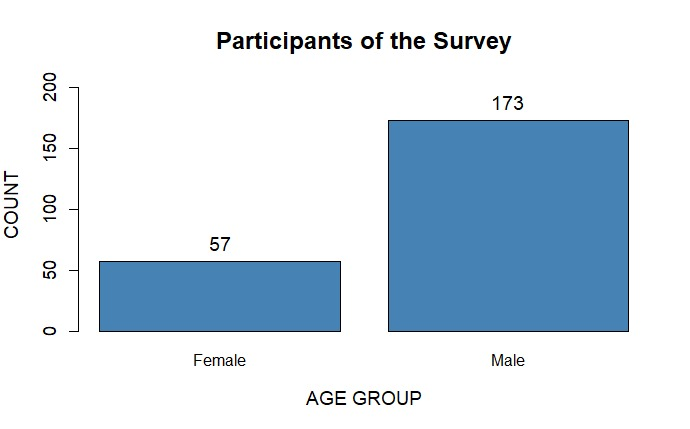
\includegraphics[width=0.7\linewidth]{IMAGES/Image 1.jpg}
	\caption{Male-Female Ratio}
	\label{G1}
\end{figure}

\

Figure \ref{G1} presents the results of a survey with $230$ participants corresponding to their genders. The figure is a Bar plot clearly representing $57$ female and $173$ male participants who took part in the survey.

\ 

\section{Employment Status}

\begin{figure}[h!]
	\centering
	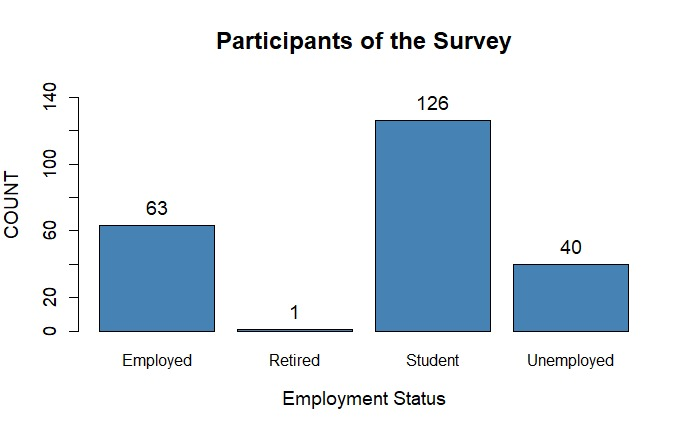
\includegraphics[width=0.75\linewidth]{IMAGES/Image 2.jpg}
	\caption{Employment Status}
	\label{G2}
\end{figure}

\ 

Figure \ref{G2} presents the results of the above-mentioned survey categorized by the
employment status of the participants. The employment status of the participants shows
that $63$ are employed, $1$ is retired, $126$ are students and $40$ are unemployed.

\ 

The survey indicates that the majority of participants are students, with a significant number
of employed and unemployed individuals and a very small representation of retired persons.
The data highlights the distribution of\\ employment status among the survey participants
and provides insights into the demographic composition of the sample.

\ 

\section{Heads in Family}

\begin{figure}[h!]
	\centering
	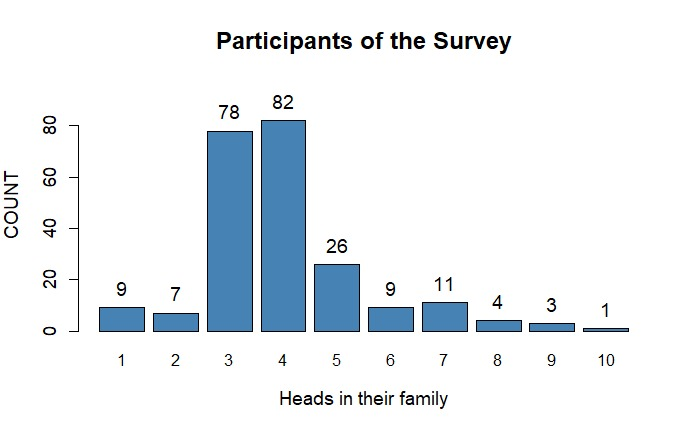
\includegraphics[width=0.75\linewidth]{IMAGES/Image 3.jpg}
	\caption{Heads in Family}
	\label{G3}
\end{figure}

\ 

In Figure \ref{G3} the document provides an overview of our survey with respect to the number of heads in the families of the participants.

\

The data indicates that the majority of participants had $3$ to $5$ members in their families,
with a few outliers having $1, 2, 6, 7, 8, 9,$ or $10$. Overall, the survey aimed to gather
information about family size within the specified sample observations.

\section{Age Group}

\begin{figure}[h!]
	\centering
	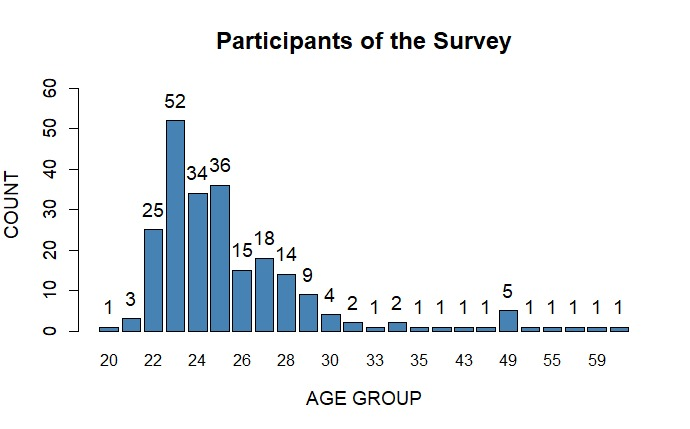
\includegraphics[width=0.8\linewidth]{IMAGES/Image 4.jpg}
	\caption{Age Group}
	\label{G4}
\end{figure}

\ 

The data represented in Figure \ref{G4} indicates the number of participants corresponding to their ages.

\ 

The data, shows that the majority of the participants, who took part in the survey, are aged between $20$ and $30$ with $52$, $34$ and $36$ persons of age $23$, $24$ and $25$ respectively. Ages of more than $34$ have been rare, although we had $5$ occurrences of age $49$ as an exception. This plot signifies that our sample data greatly consists observations of people having age between $20$ and $30$.